\ifdefined\included
\else
\setcounter{chapter}{8} %% Numéro du chapitre précédent ;)
\dominitoc
\faketableofcontents
\fi

\chapter{A robot in the mall: The MuMMER project}
\minitoc

This chapter is a sum-up of an article submitted to the  User Modeling and User-Adapted Interaction (UMUAI) Journal. This work has been achieved in collaboration with Amandine Mayima, Guilhem Buisan, Phani-TejaSingamaneni, Yoan Sallami, KathleenBelhassein, and Jules Waldhart. In this chapter, we first give an overview of the European H2020 Project \acrfull{mummer}\footnote{http://mummer-project.eu/}, in the context of which the contribution of chapter~\ref{chap:3} was made. We then present the components developed by the LAAS-RIS team with a focus on the component in which I participated as well as their integration in a robotic architecture.

\section{Introduction}

In large scale, indoor environments, like museums, shopping malls, or airports, the presence of large interactive screens, maps, or signs underline the importance of providing information on itineraries. However, reading such maps can be challenging and some information can be missing like the location of the shops selling a given product. To bring such new information and help people to find their itinerary in large indoor environments such as shopping malls, robots can be used.

To study this challenge and the underlined Human-Robot Interaction requirement, in the context of the European H2020 Project \acrshort{mummer}, we have developed and deployed a social service robot in one of the largest malls of Finland, Ideapark in the city of Lemp\"a\"al\"a. The resulting robot is able to chat with customers and guide them. The chatting has been brought by a partner of the project. The contribution of the LAAS-RIS team, and thus the focus of this chapter, was on the direction-giving task.

With a mall having approximately 1.2 kilometers of pedestrian streets and more than 150 shops, having a robot accompanying customers would be time-consuming. Taking inspiration from the mall employees, we chose to verbally describe the route while grounding it with pointing gestures. The robot can however move a few meters if needed. %Such a movement can be useful to improve the perspective sharing of landmark to better ground the route description.
The output of this project is a complete robot architecture that integrates a number of components. Each of them makes use of various models and decisional algorithms, all integrating explicitly human models.

First, we provide background information about robot guides and discuss how the human partner has been considered. Then, we present the human-human exploratory studies used to identify the required abilities for a guide robot. We then present the developed architecture and its components. We end this chapter with integration on a real robotic system with some detail on its deployment "into the wild".

\section{Related work}

\section{Learning from pilot-studies}

\begin{figure}[ht!]
\centering
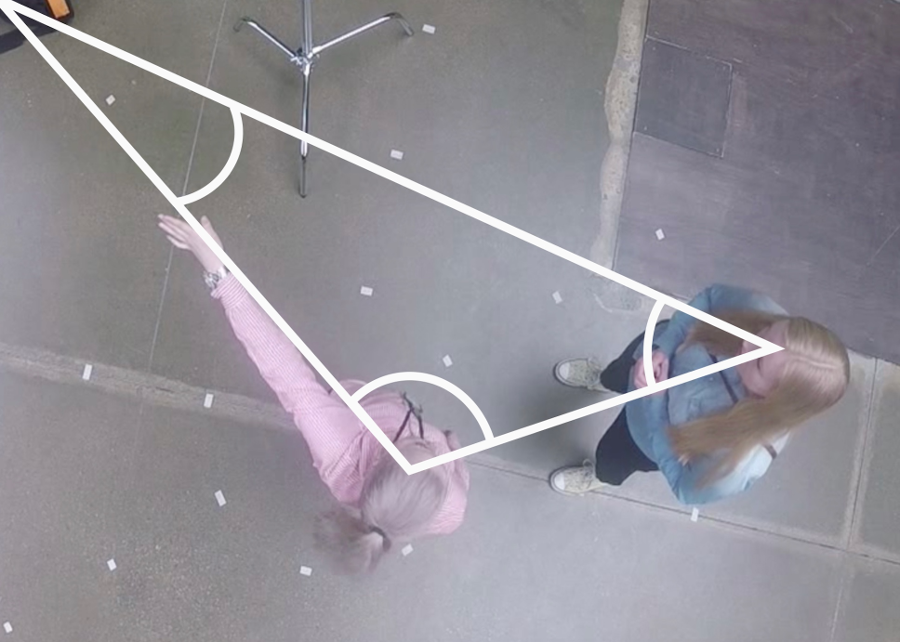
\includegraphics[scale=0.35]{figures/chapter8/human_guide.png}
\caption{\label{fig:chap8_human_guide} todo. }
\end{figure}

\section{The deliberative architecture}

\begin{figure}[ht!]
\centering
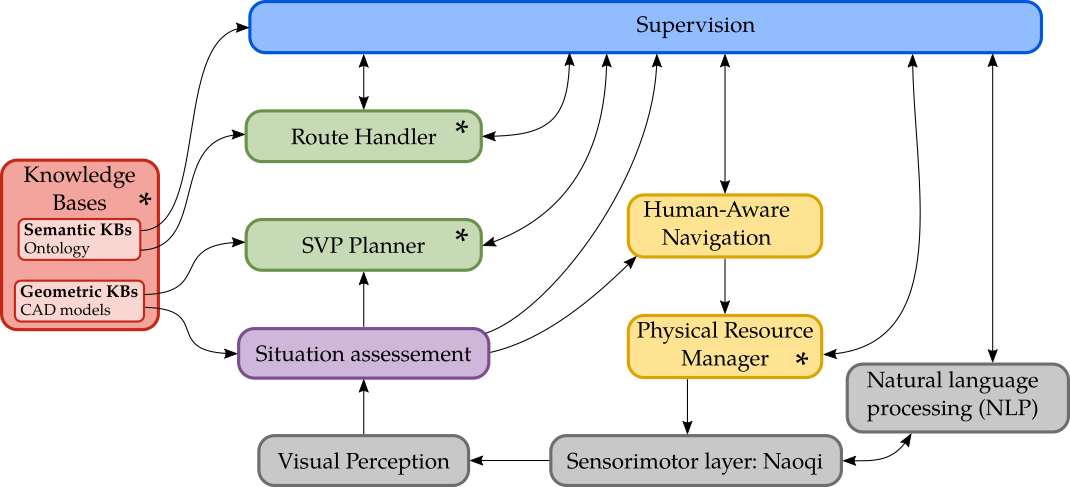
\includegraphics[width=\textwidth]{figures/chapter8/architecture.png}
\caption{\label{fig:chap8_architecture} todo. }
\end{figure}

\subsection{Environment representation}

\subsubsection{Geometric representation}

\begin{figure}[ht!]
\centering
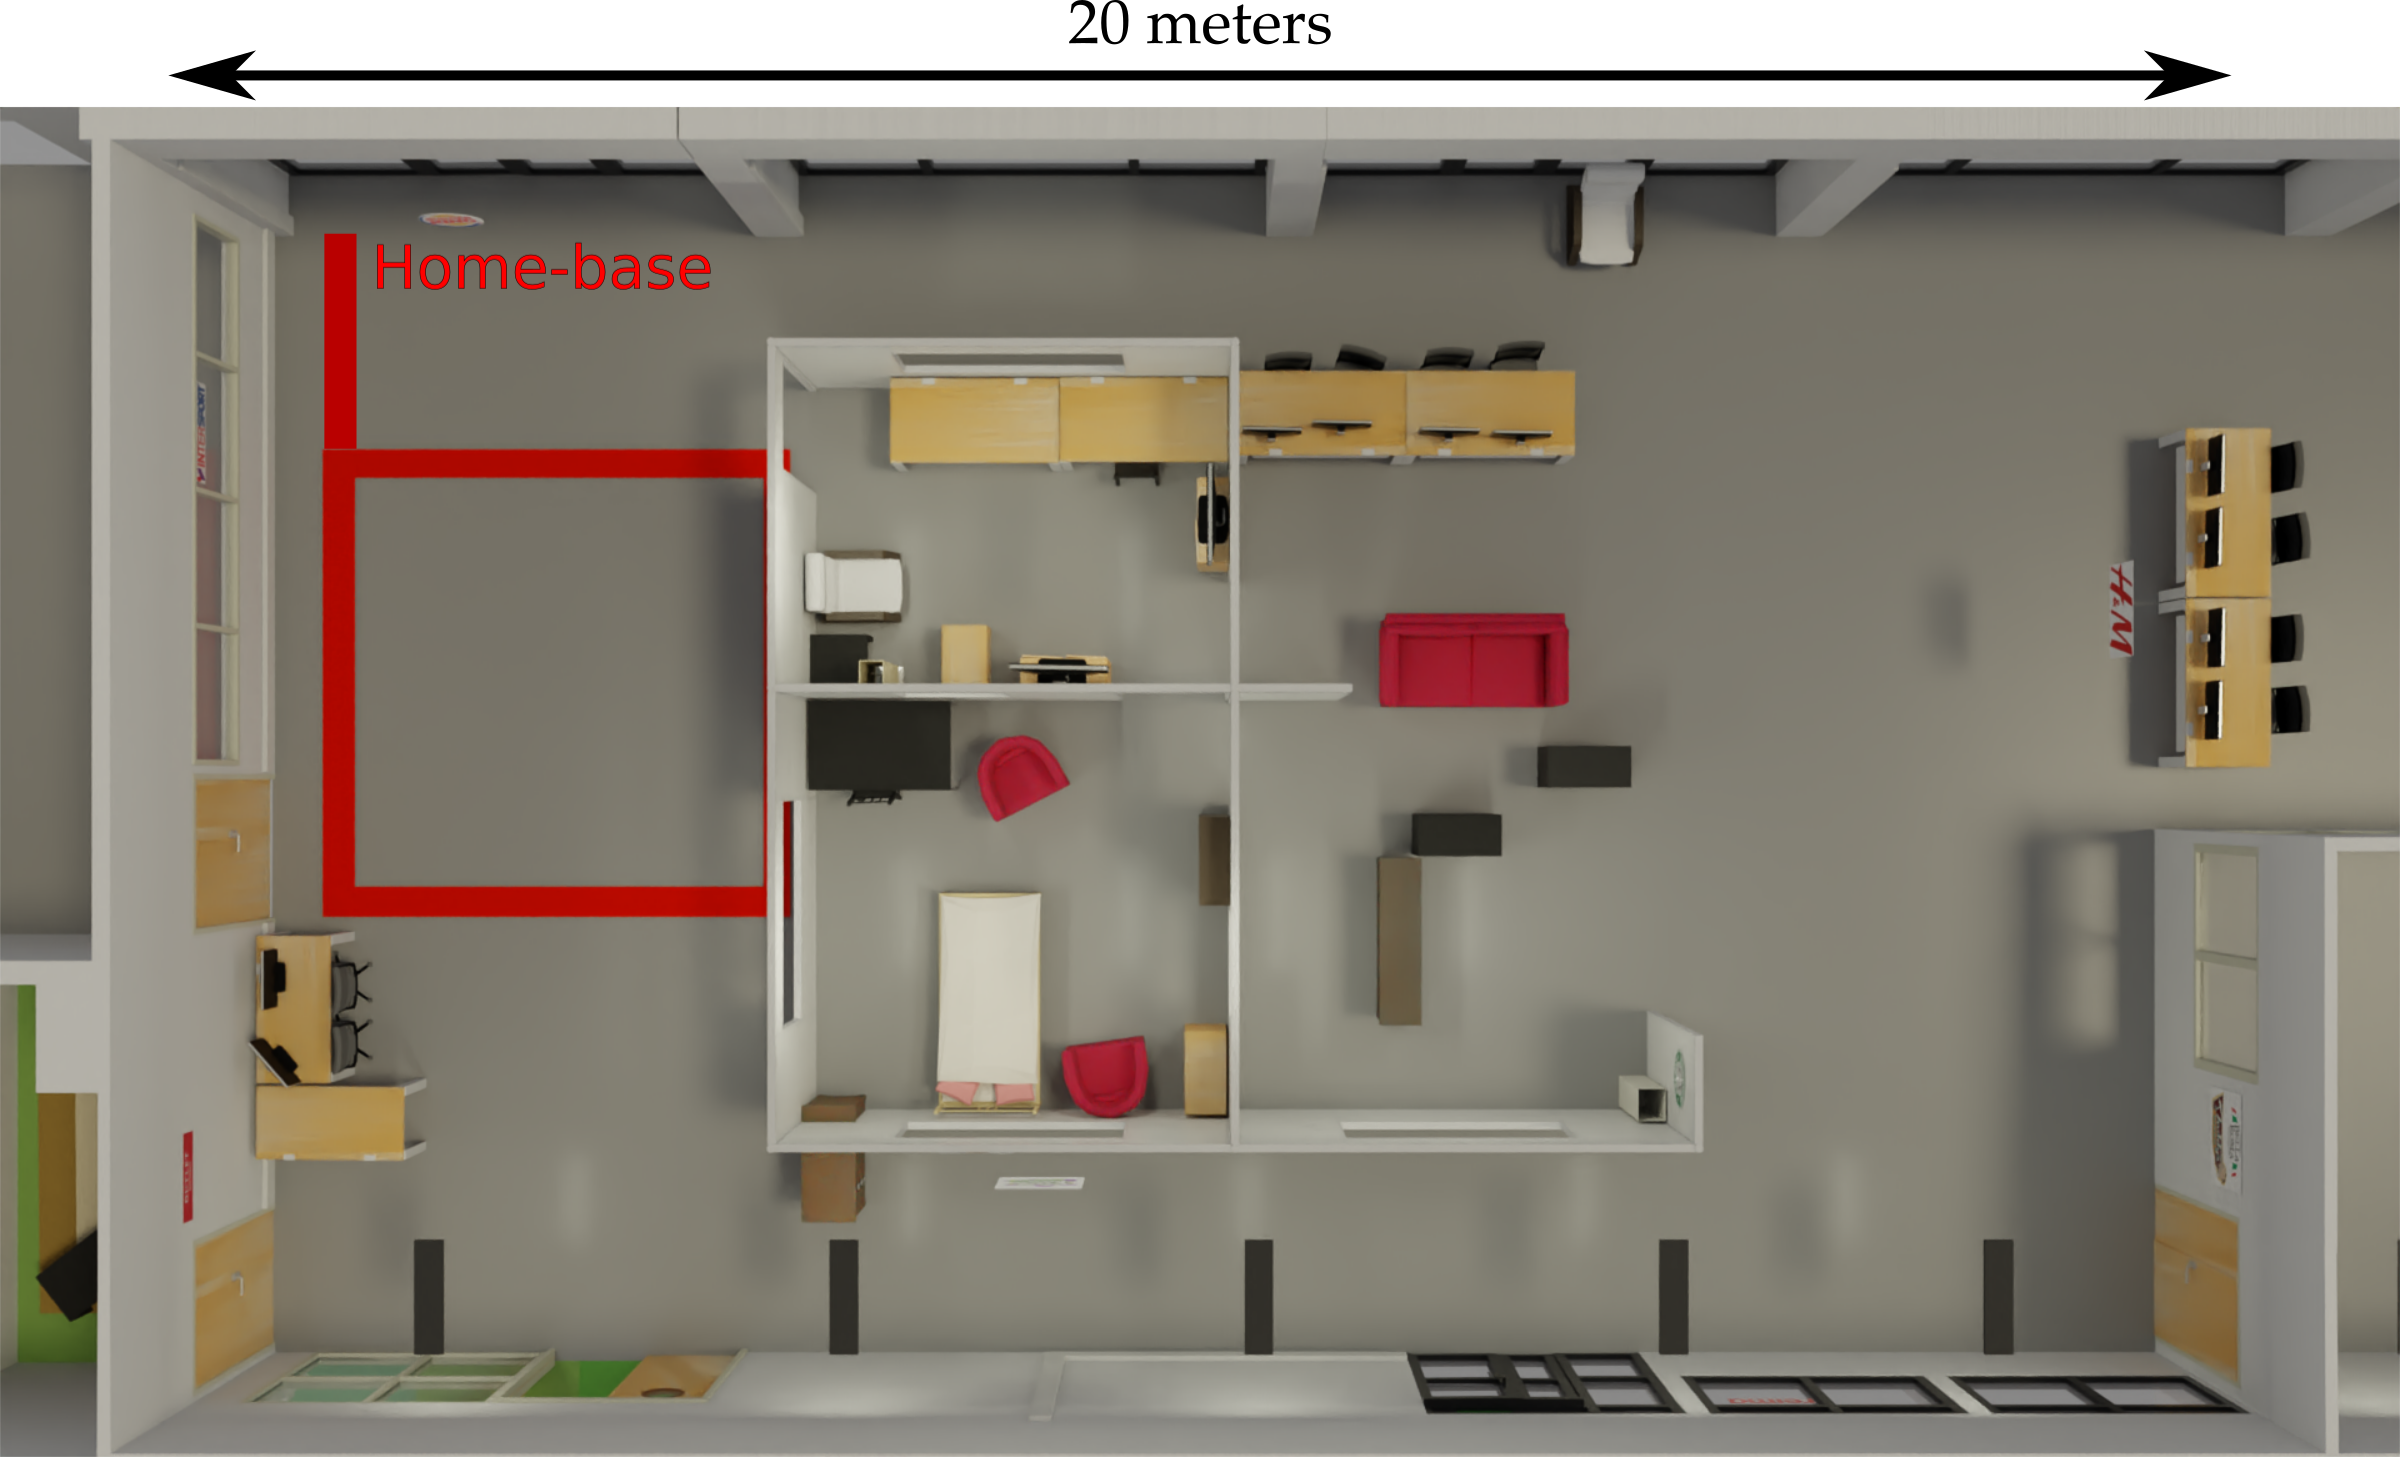
\includegraphics[scale=0.15]{figures/chapter8/adream_base_m.png}
\caption{\label{fig:chap8_adream_base} todo. }
\end{figure}

\begin{figure}[ht!]
\centering
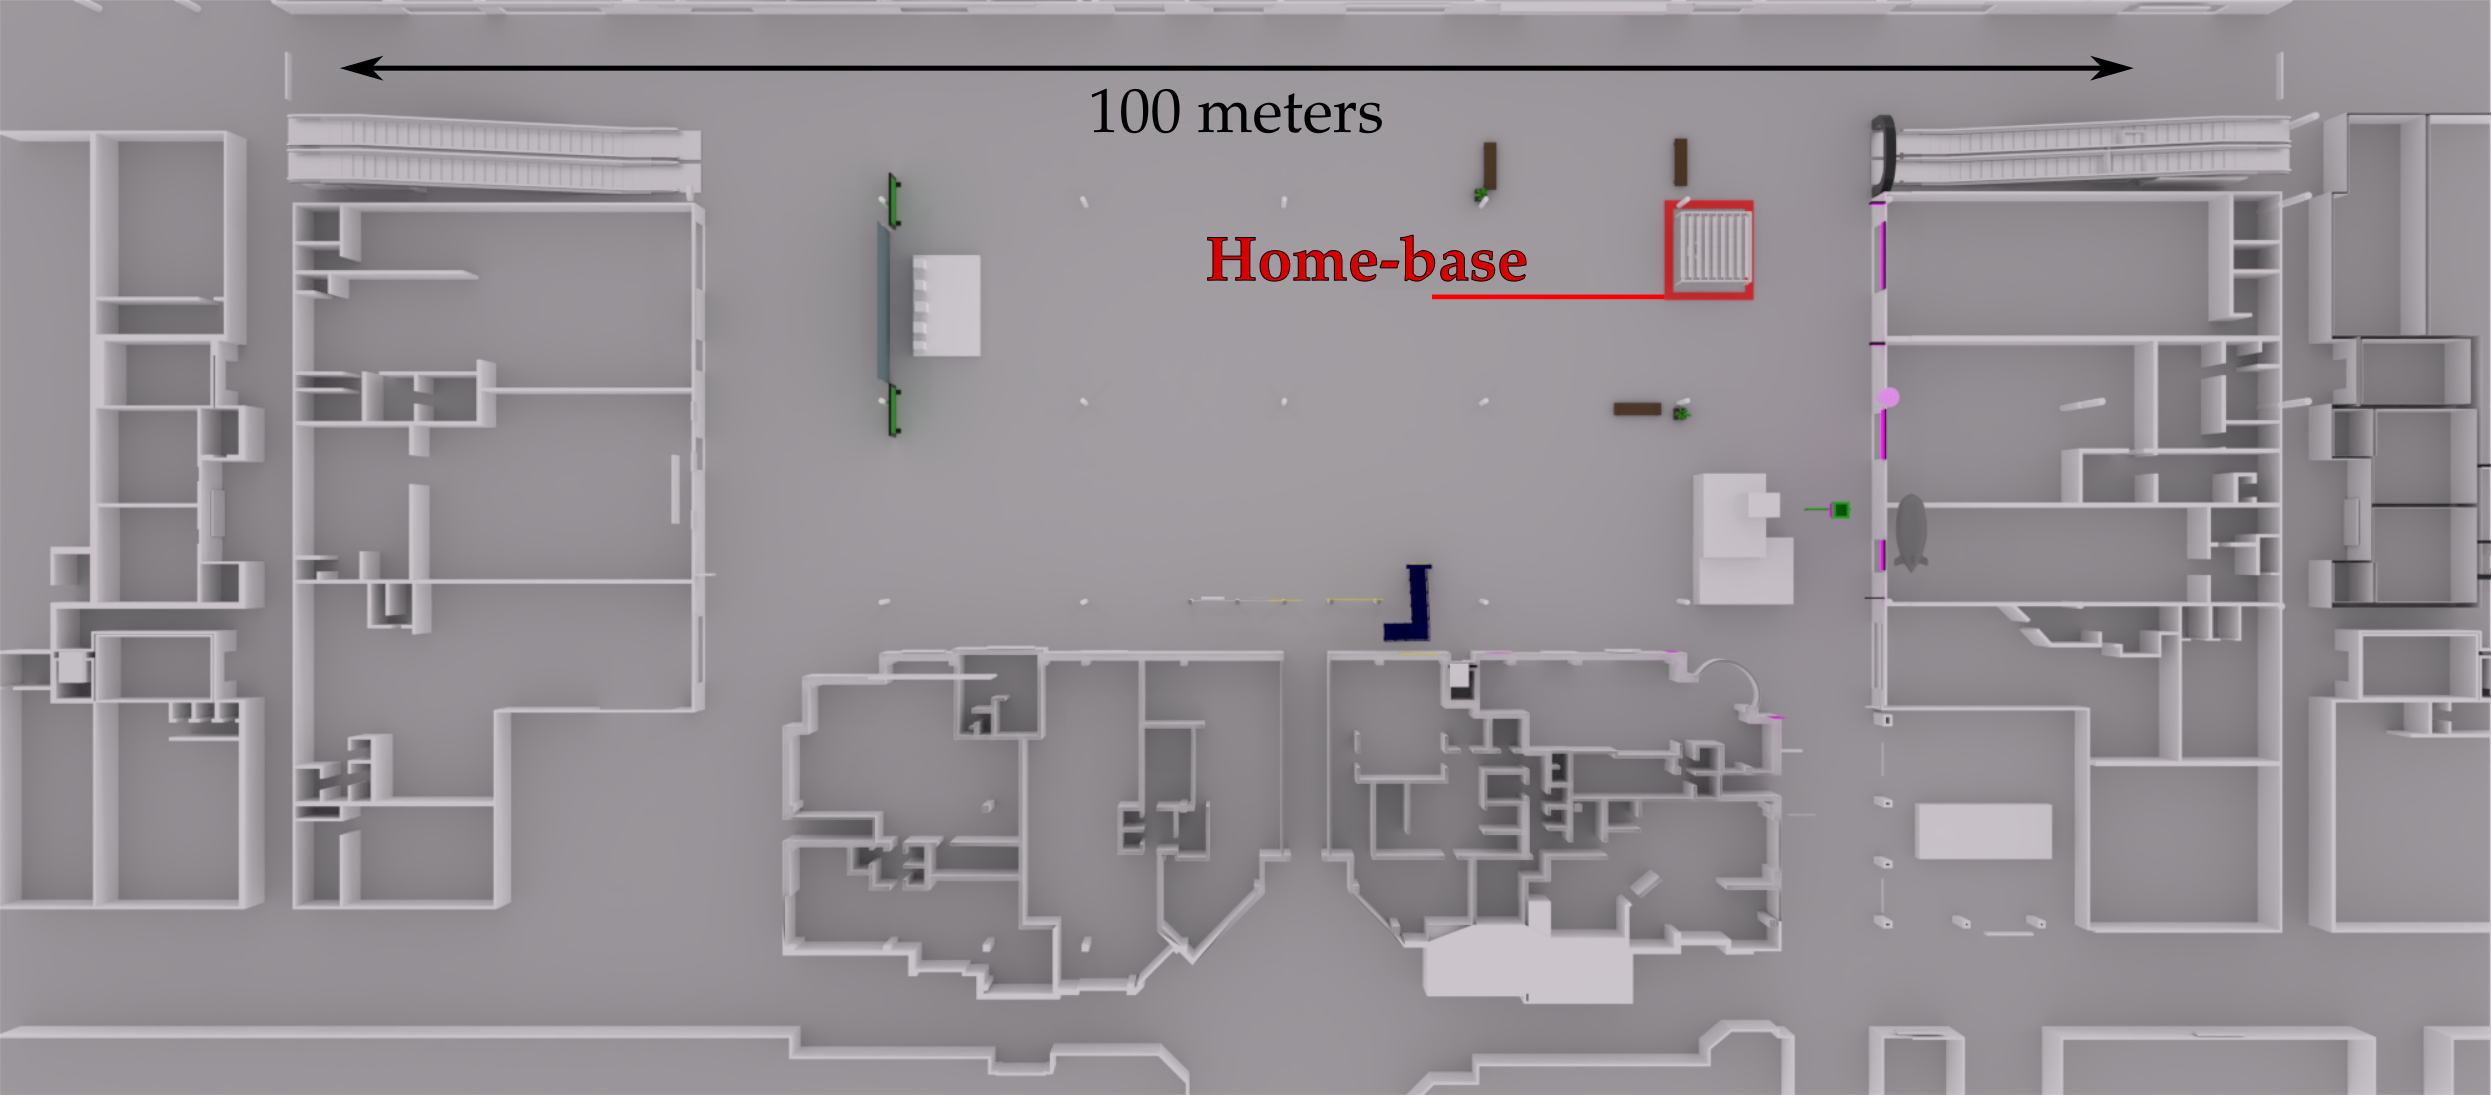
\includegraphics[scale=0.15]{figures/chapter8/ideapark_base_m.png}
\caption{\label{fig:chap8_ideapark_base} todo. }
\end{figure}

\subsubsection{Semantic representation}

\begin{figure}[ht!]
\centering
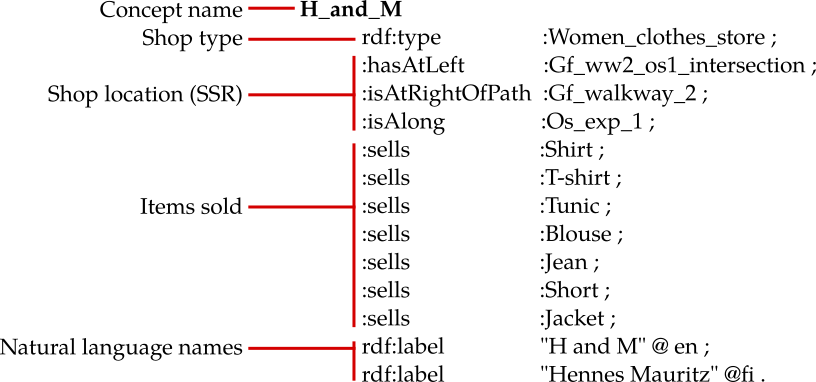
\includegraphics[scale=0.45]{figures/chapter8/zizzi.png}
\caption{\label{fig:chap8_zizzi} todo. }
\end{figure}

\subsection{Perceiving the partner}

\subsection{Generating route description}

\subsection{Planning a shared visual perspective}

\begin{figure}[ht!]
\centering
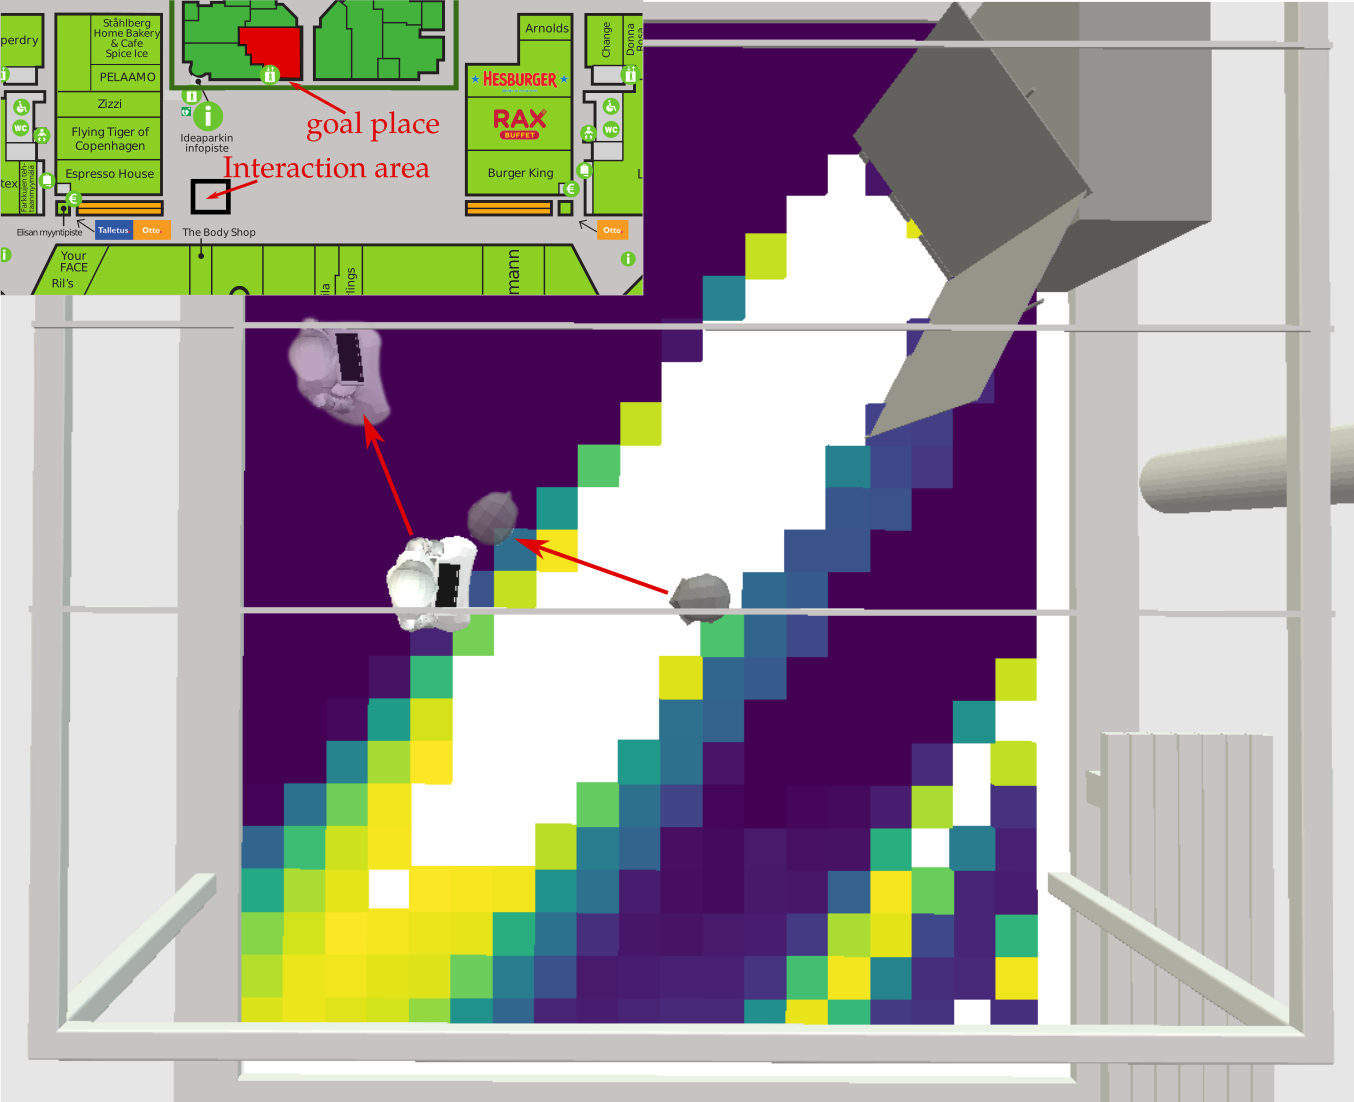
\includegraphics[scale=0.25]{figures/chapter8/grid_map.png}
\caption{\label{fig:chap8_svp_grid} todo. }
\end{figure}

\begin{figure}[ht!]
\centering
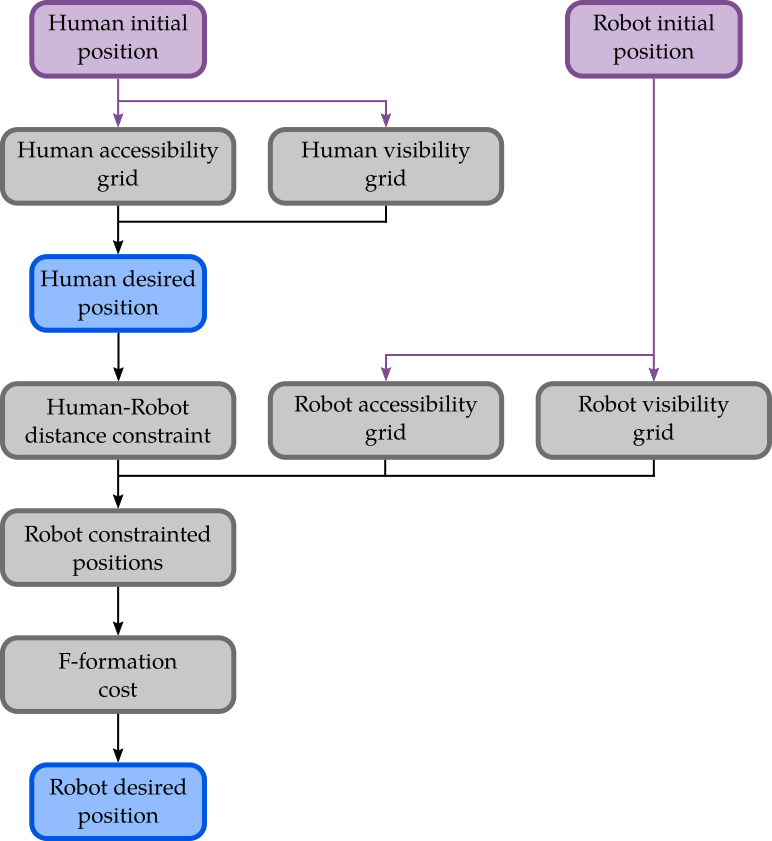
\includegraphics[scale=0.45]{figures/chapter8/svp.png}
\caption{\label{fig:chap8_svp} todo. }
\end{figure}

\subsection{Navigate close to the human}

\subsection{Executing and controling the task}

\section{Embody architecture in a physical robot}

\subsection{Pepper in Ideapark}

\begin{figure}[ht!]
\centering
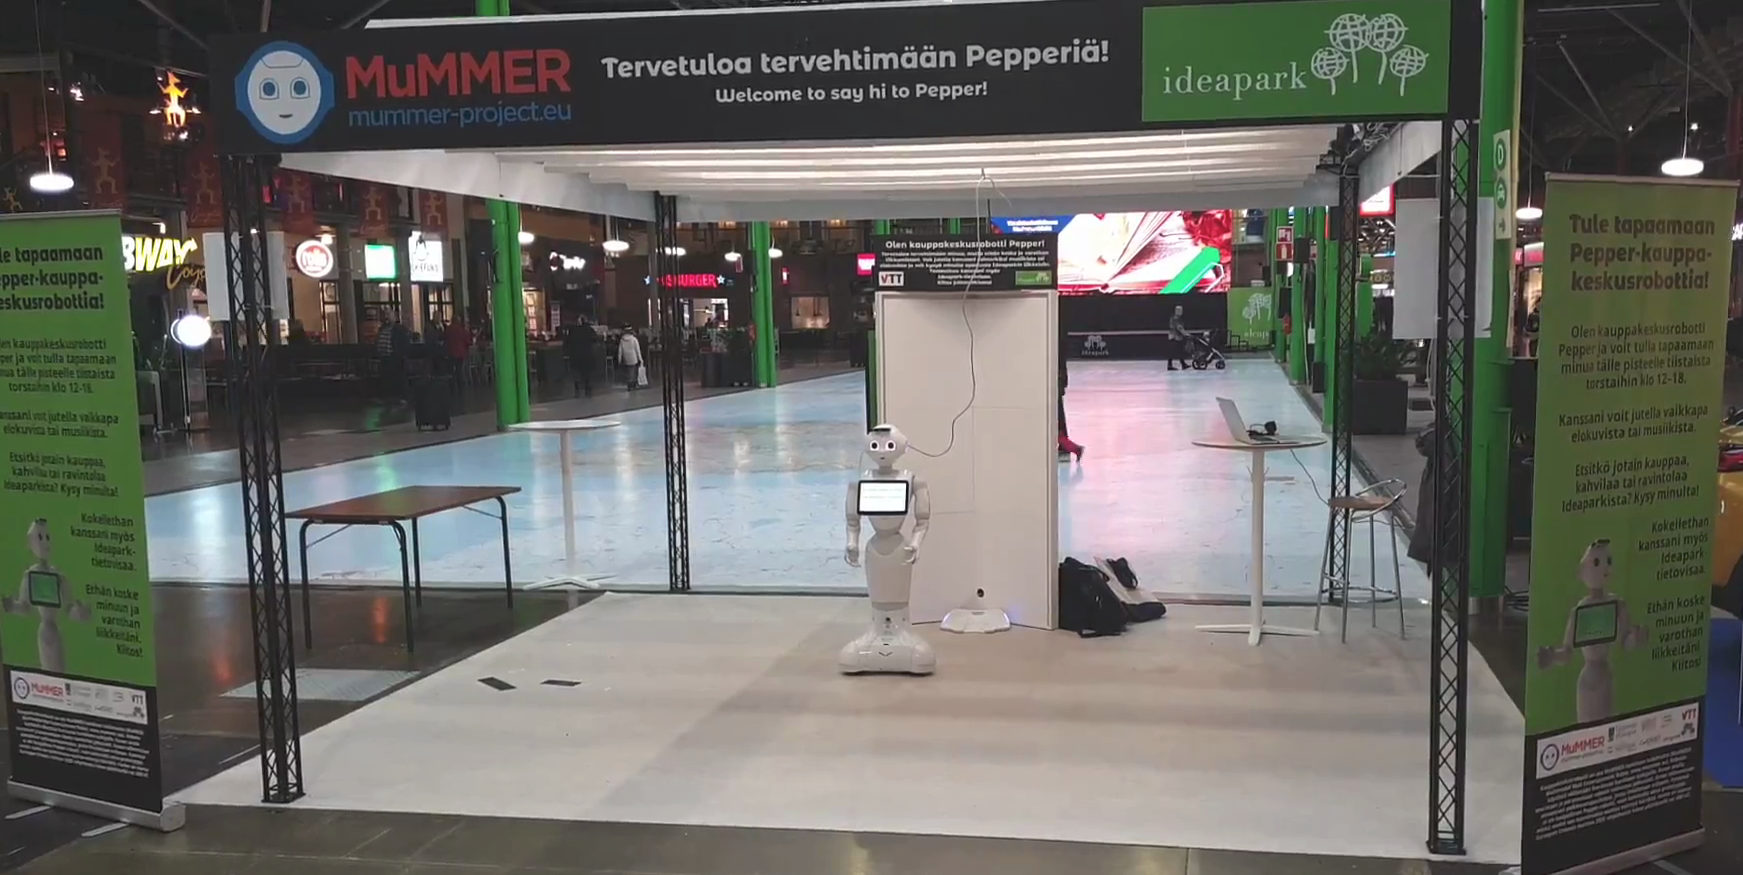
\includegraphics[scale=0.15]{figures/chapter8/pepper_mall.png}
\caption{\label{fig:chap8_pepper_mall} todo. }
\end{figure}

\subsection{Pepper "in the wild"}